\begin{figure*}[t]
\centering
\begin{subfigure}[b]{0.333\textwidth}
       \centering
        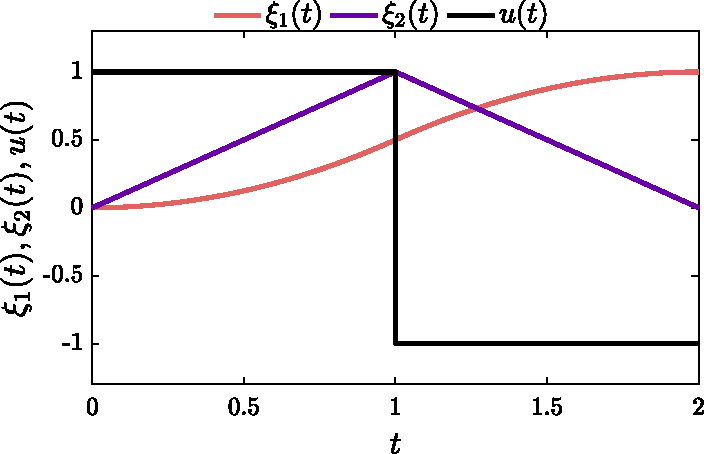
\includegraphics[width=\textwidth]{../ch3/figures/sasa_1.pdf}
        \caption{$k=0$.\label{fig:ch3:sasa_1}}
\end{subfigure}% 
\begin{subfigure}[b]{0.333\textwidth}
       \centering
        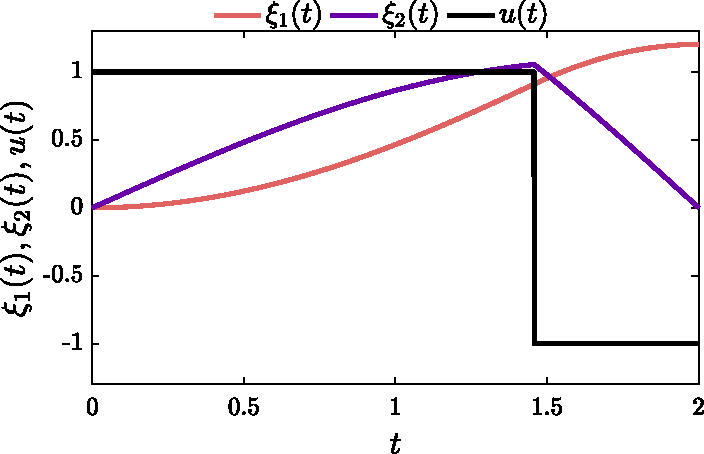
\includegraphics[width=\textwidth]{../ch3/figures/sasa_2.pdf}
        \caption{$k^*=0.8547$.\label{fig:ch3:sasa_2}}
\end{subfigure}%
\begin{subfigure}[b]{0.333\textwidth}
       \centering
        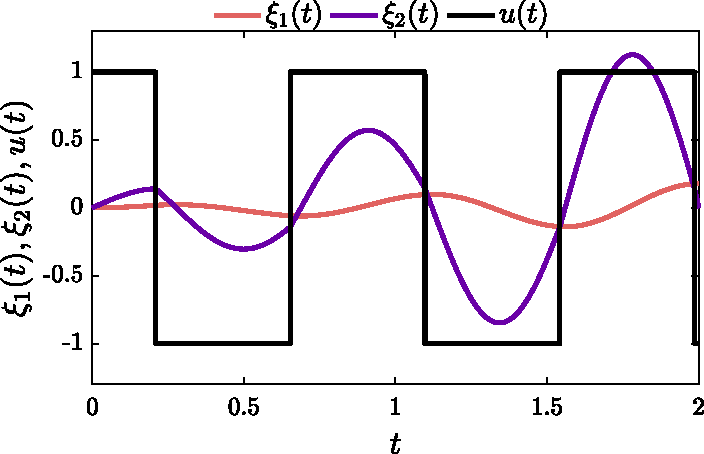
\includegraphics[width=\textwidth]{../ch3/figures/sasa_3.pdf}
        \caption{$k=50$.\label{fig:ch3:sasa_3}}
\end{subfigure}%
\caption[Simple SASA test problem (TP3) results]{Simple SASA test problem (TP3) results with $J=1$, $t_f=2$, and $u_{\max}=1$.\label{fig:ch3:sasa}}
\end{figure*}